\chapter{Analiza dynamiczna}\label{chap:dynamic}

W tym rozdziale przedstawiono analizę wariantu dynamicznego, w którym struktura grafu zmienia się w czasie. Motywacją jest realizm: sieci znajomych i zespoły w firmie ewoluują — pojawiają się nowe osoby, inne odchodzą, powstają lub zanikają połączenia. W takich warunkach algorytm powinien nie tylko znaleźć dobre rozwiązanie początkowe, lecz także utrzymywać niskie koszty w kolejnych krokach przy umiarkowanych nakładach czasowych.

\section{Założenia i model zmian}

Symulacja dynamiki oparta jest o moduł \texttt{glopt.dynamic\_simulator} oraz skrypt uruchomieniowy \texttt{src/glopt/cli/dynamic.py}. W każdym kroku stosowane są mutacje grafu sterowane parametrami \texttt{MutationParams}: prawdopodobieństwa dodania/usupełnienia wierzchołków i krawędzi oraz limity maksymalnej liczby zmian na krok. W badaniu zastosowano parametry (por. \texttt{dynamic.py}):
\begin{itemize}
  \item \texttt{ADD\_NODES\_PROB} = 0.06, \texttt{REMOVE\_NODES\_PROB} = 0.04
  \item \texttt{ADD\_EDGES\_PROB} = 0.18, \texttt{REMOVE\_EDGES\_PROB} = 0.12
  \item limity zmian skalowane do rozmiaru bieżącego grafu (dopełnienie w krawędziach zależy od aktualnej liczby krawędzi)
\end{itemize}
Po mutacjach wykonywane jest \emph{rebalance} — ponowne wyznaczenie grup licencyjnych. Dla części metaheurystyk (genetyczny, wyżarzanie, tabu, mrówkowy) wykorzystuje się \emph{warm start}, tj. projekcję poprzedniego rozwiązania jako inicjalizacji. Pozostałe algorytmy uruchamiane są \emph{cold}.

\paragraph{Parametry przebiegu} Liczba kroków symulacji \texttt{NUM\_STEPS} wynosi domyślnie 50. Dla serii z małym grafem (\texttt{dynamic\_20}) wykonano 100 kroków, aby wyraźniej uchwycić zjawiska w dłuższym horyzoncie. Badano trzy rodziny grafów syntetycznych: \texttt{random}, \texttt{small\_world}, \texttt{scale\_free}. Zestawy licencji: \texttt{duolingo\_super}, \texttt{roman\_domination} oraz warianty parametryczne \texttt{roman\_p\_x}. Zestaw \texttt{spotify} nie jest omawiany w tym rozdziale.

\section{Zbiory danych i organizacja wyników}

Analizowane pliki CSV:
\begin{itemize}
  \item \texttt{runs/dynamic\_20/csv/20250905\_185404\_dynamic.csv} — stały rozmiar około $n\approx20$ niesion w trakcie zmian, $100$ kroków; pełny przekrój algorytmów i wariantów licencji (w tym \texttt{roman\_p\_x}).
  \item \texttt{runs/20250907\_014311\_dynamic/csv/20250907\_014311\_dynamic.csv} — rozmiary $n\in\{40,80,\dots,10000\}$, $50$ kroków; dla $n>20$ ograniczono się do \texttt{duolingo\_super} i \texttt{roman\_domination}.
\end{itemize}
Skrypt \texttt{scripts/analysis/dynamic\_analysis.py} generuje wykresy per (licencja, typ grafu, algorytm): koszt całkowity i czas w funkcji kroku, a także zagregowaną intensywność mutacji. Wykresy zapisano w katalogu \texttt{docs/thesis/assets/figures/dynamic/}.

\section{Intensywność mutacji}

Na rysunkach \ref{fig:dyn20_mut} i \ref{fig:full_mut} pokazano średnią liczbę zmian (dodane/uszunięte wierzchołki i krawędzie) przypadającą na wiersz danych w danym kroku. Losowe wyzwalanie mutacji z zadanymi prawdopodobieństwami powoduje umiarkowaną, ale stałą presję zmian w czasie.

\begin{figure}[H]
  \centering
  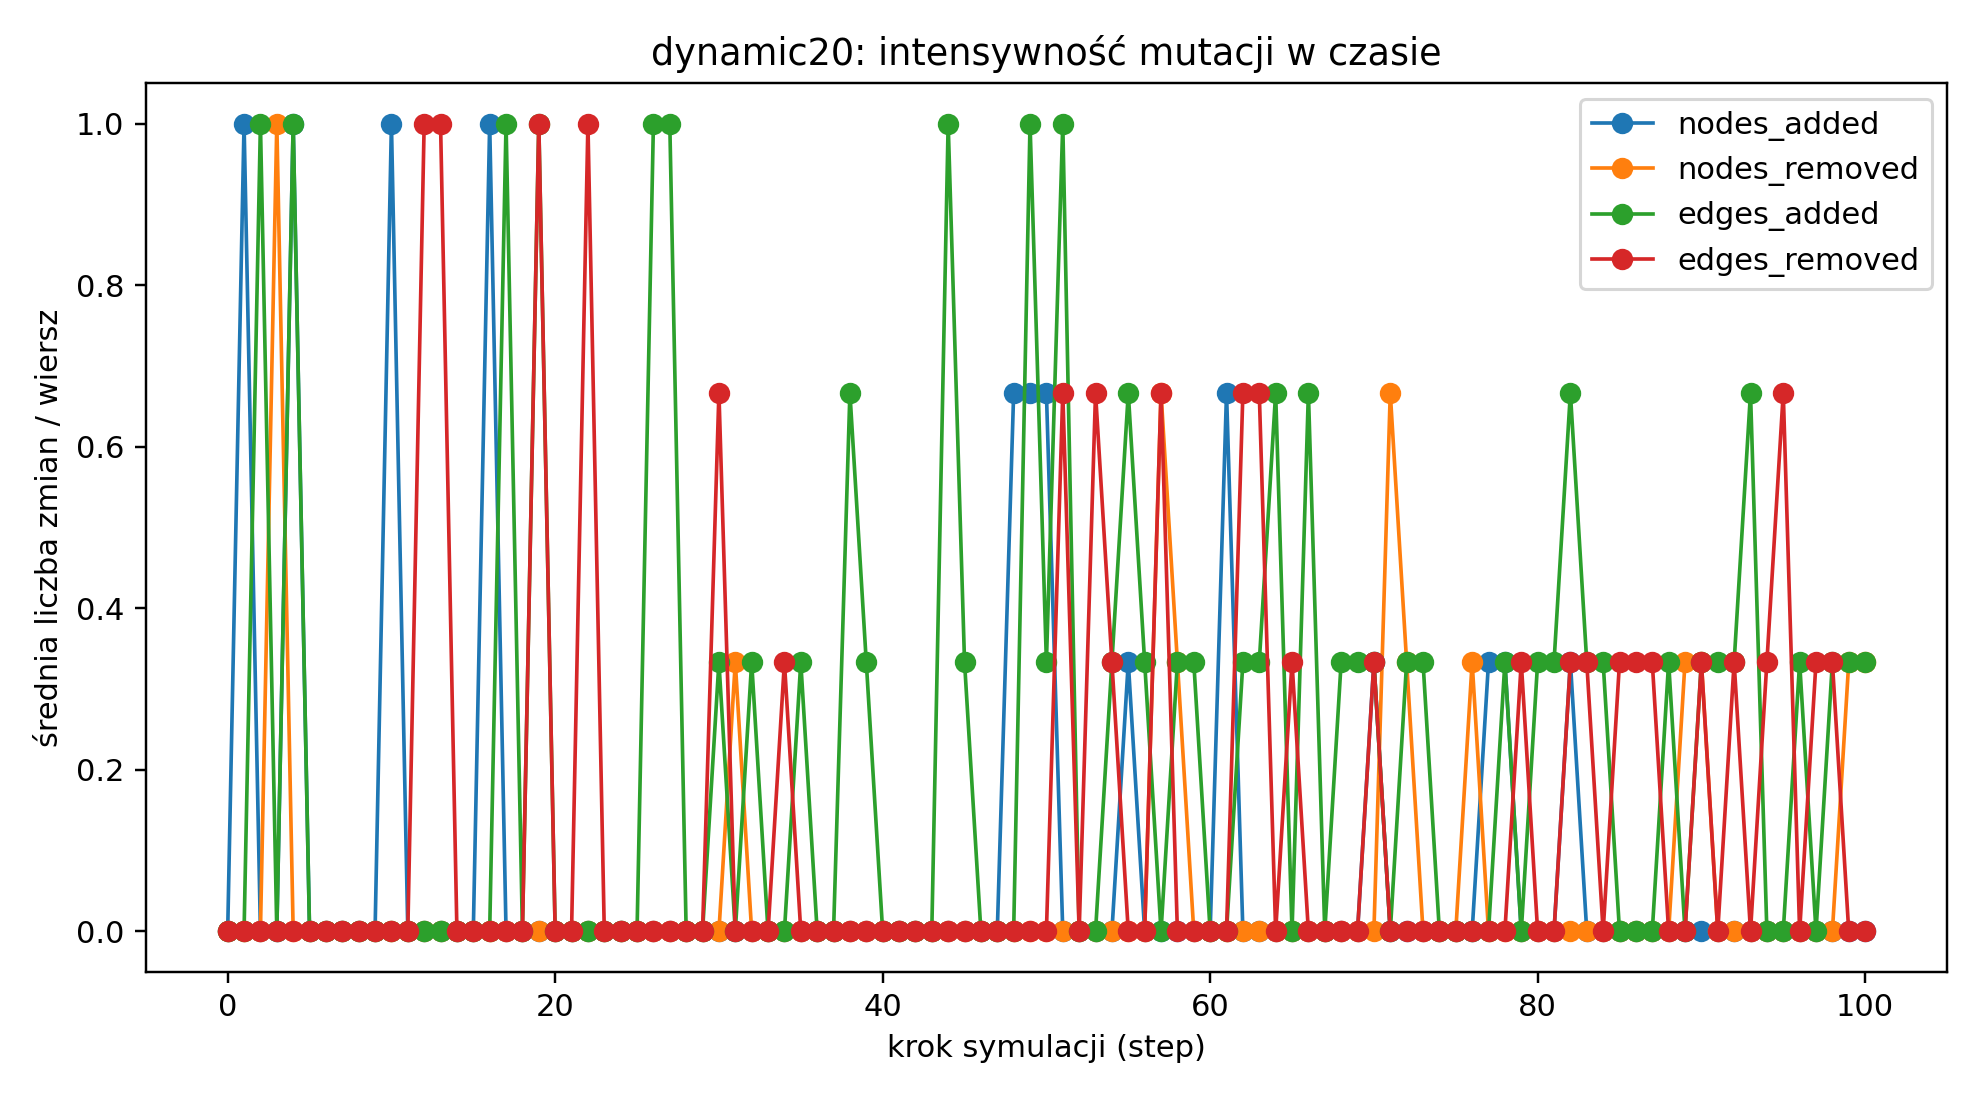
\includegraphics[width=0.75\linewidth]{assets/figures/dynamic/dynamic20_mutation_intensity.png}
  \caption{\texttt{dynamic\_20}: intensywność mutacji w czasie (średnia na wiersz).}
  \label{fig:dyn20_mut}
\end{figure}

\begin{figure}[H]
  \centering
  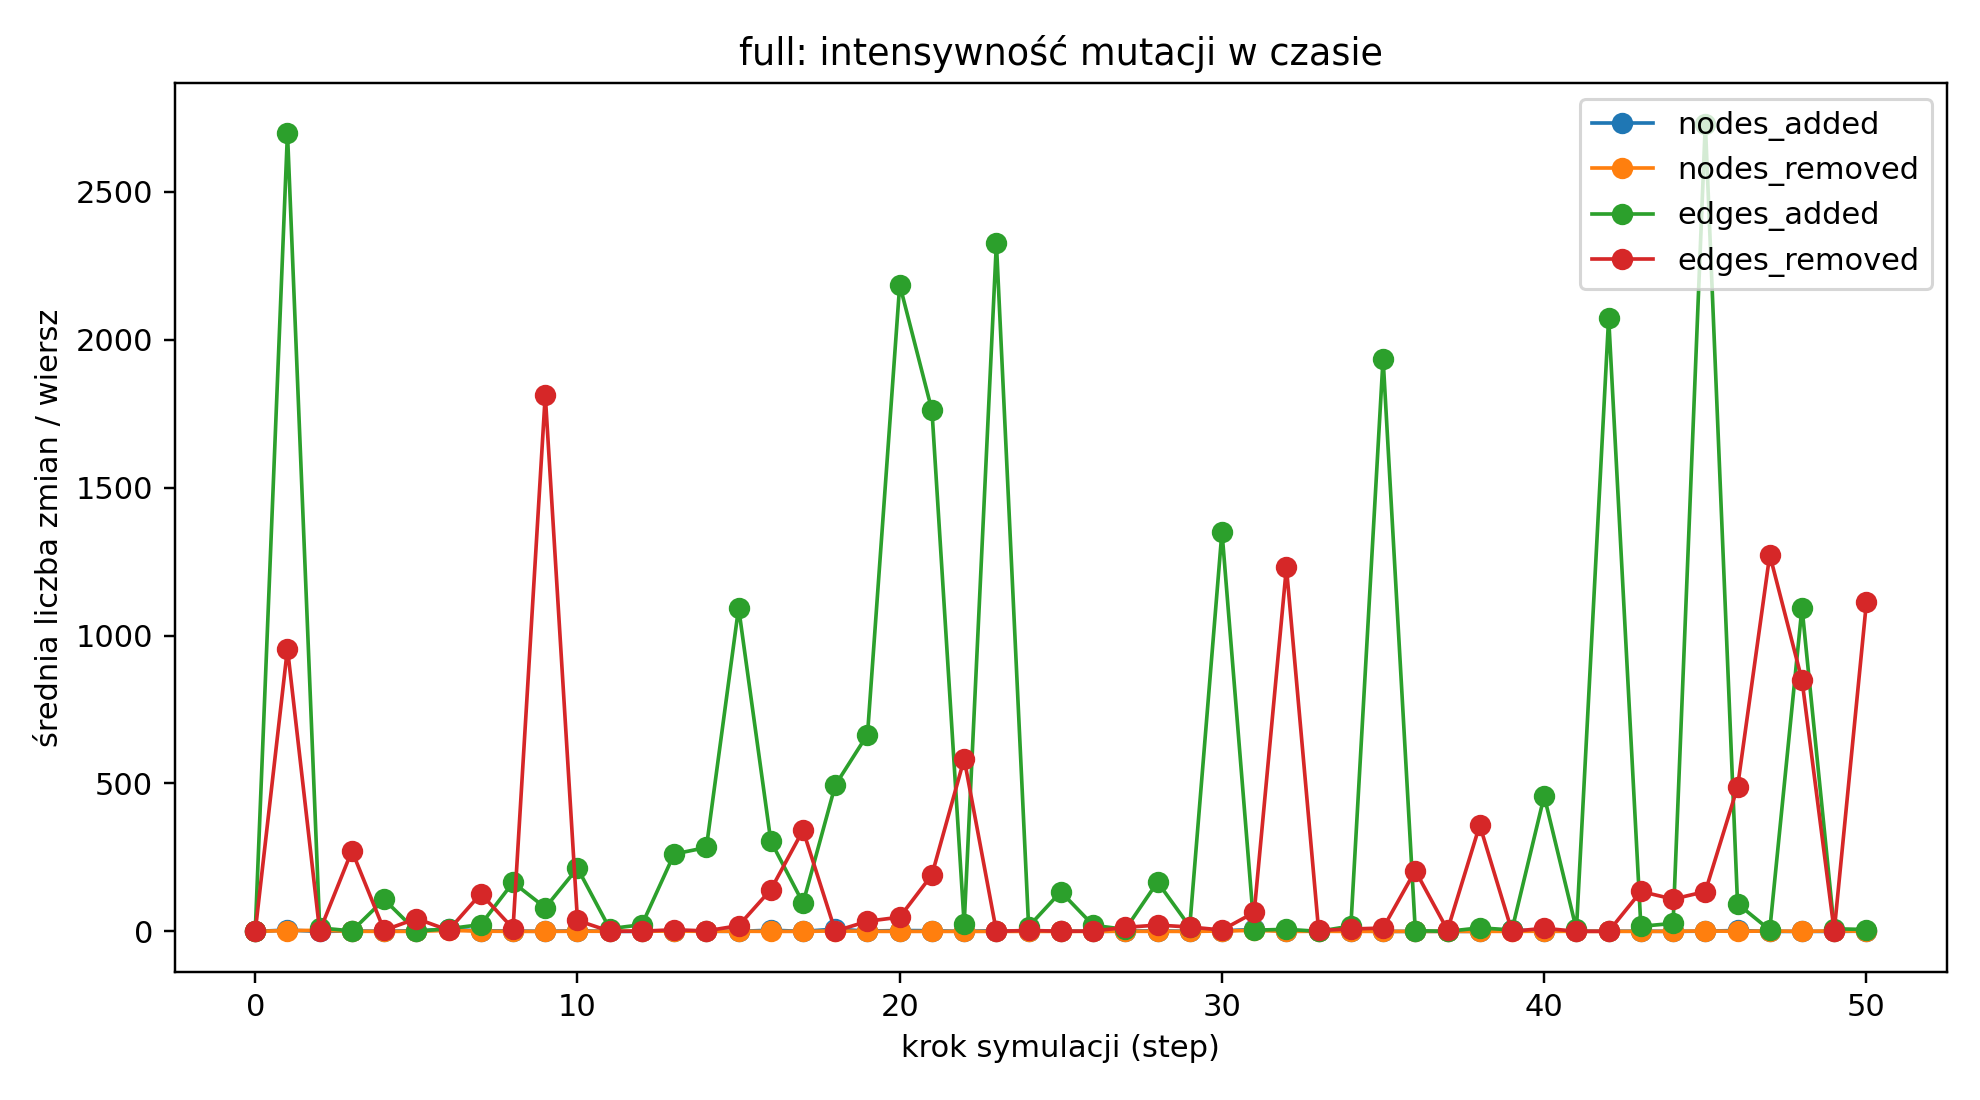
\includegraphics[width=0.75\linewidth]{assets/figures/dynamic/full_mutation_intensity.png}
  \caption{\texttt{full}: intensywność mutacji w czasie (średnia na wiersz).}
  \label{fig:full_mut}
\end{figure}

\section{Trajektorie kosztu i czasu}

Poniżej przedstawiono przykładowe trajektorie dla wybranych algorytmów. Linie pokazują wartość metryki w kolejnych krokach dla danego typu grafu i konfiguracji licencji.

\subsection{\texttt{dynamic\_20}: \texttt{duolingo\_super}, graf \texttt{random}}

\begin{figure}[H]
  \centering
  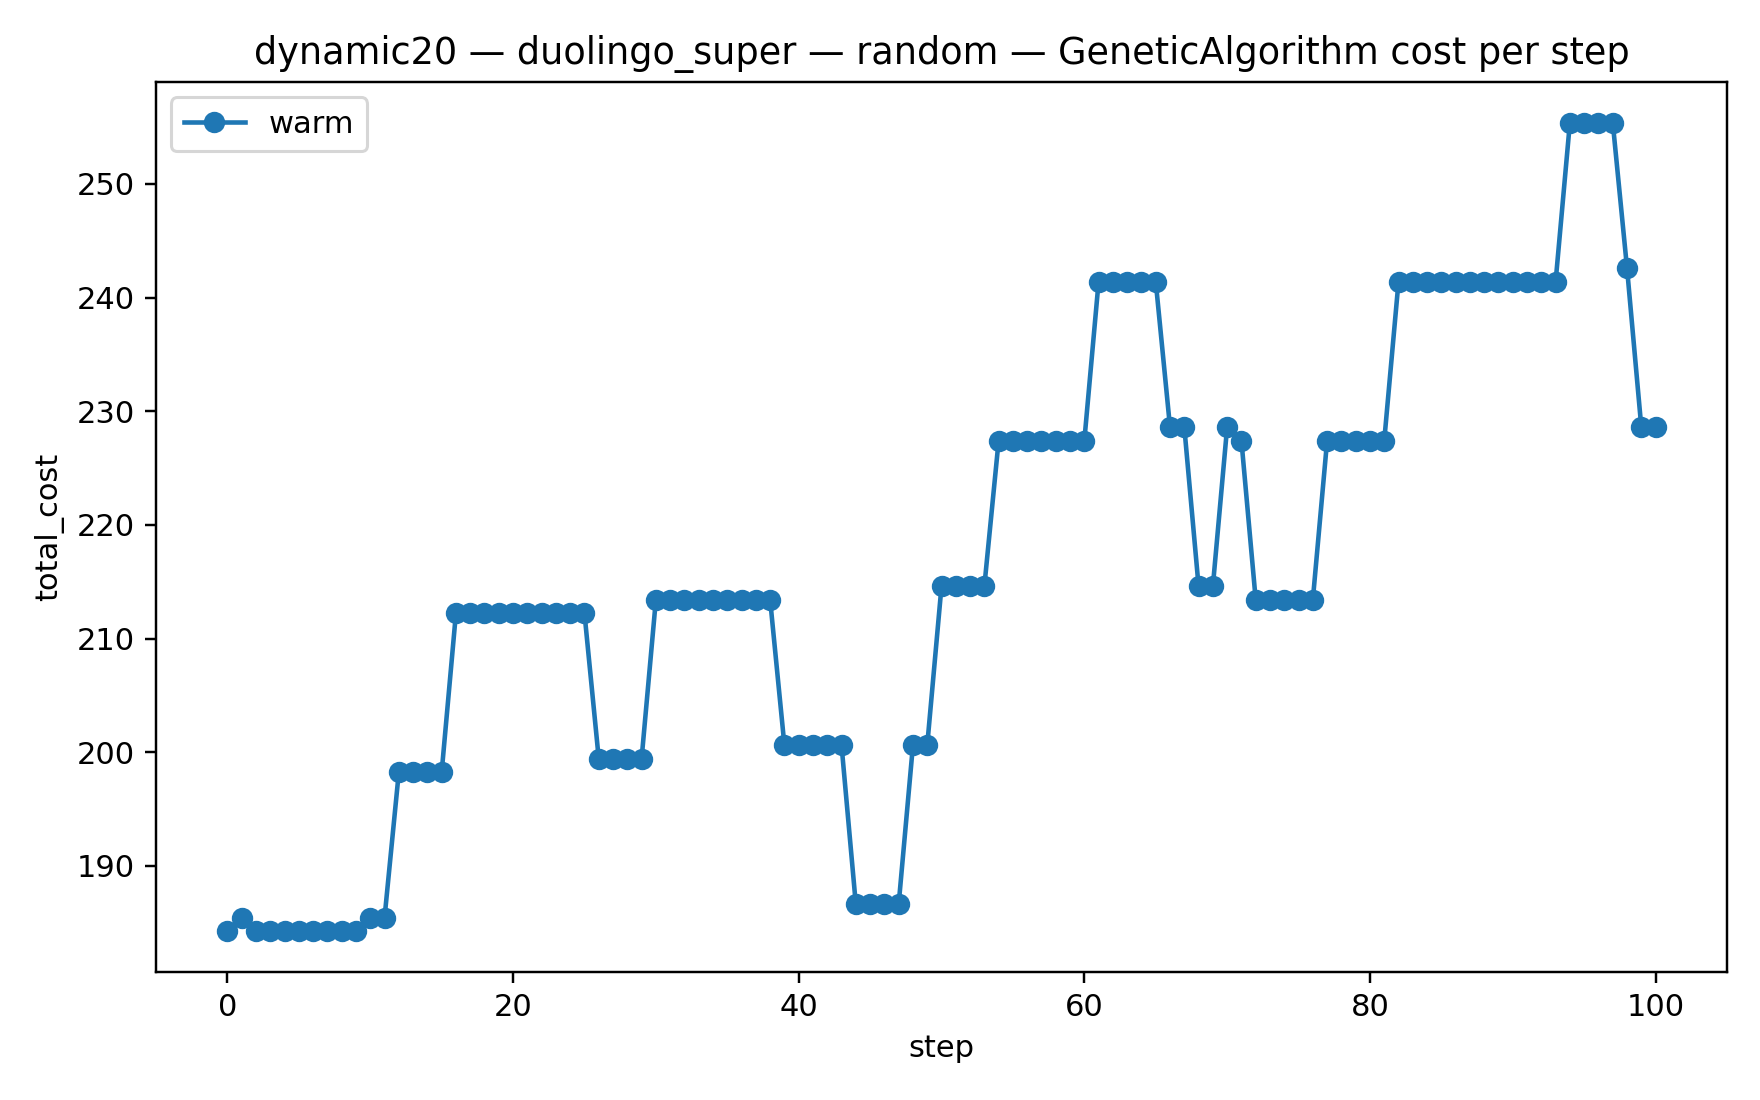
\includegraphics[width=0.48\linewidth]{assets/figures/dynamic/dynamic20/duolingo_super/random/GeneticAlgorithm_cost_per_step.png}
  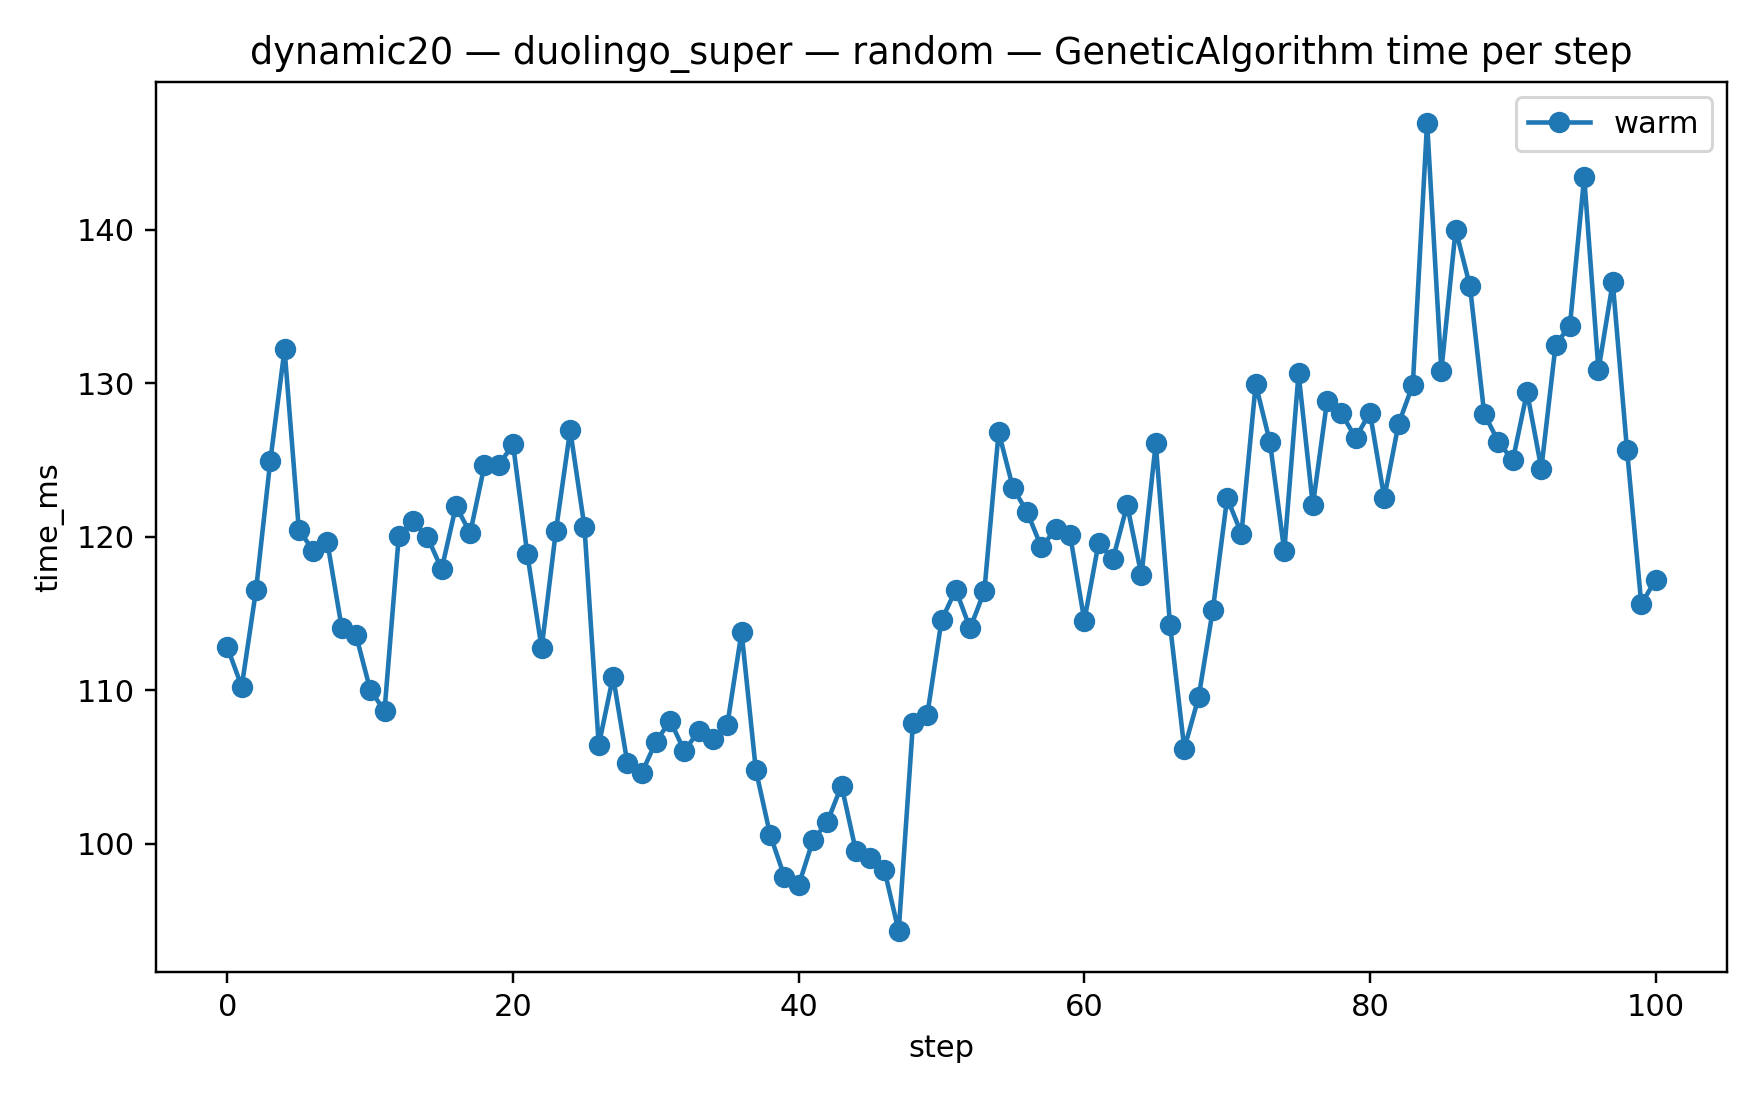
\includegraphics[width=0.48\linewidth]{assets/figures/dynamic/dynamic20/duolingo_super/random/GeneticAlgorithm_time_per_step.png}
\caption{Algorytm genetyczny (warm start): koszt i czas vs krok.}
  \label{fig:dyn20_duo_genetic}
\end{figure}

\begin{figure}[H]
  \centering
  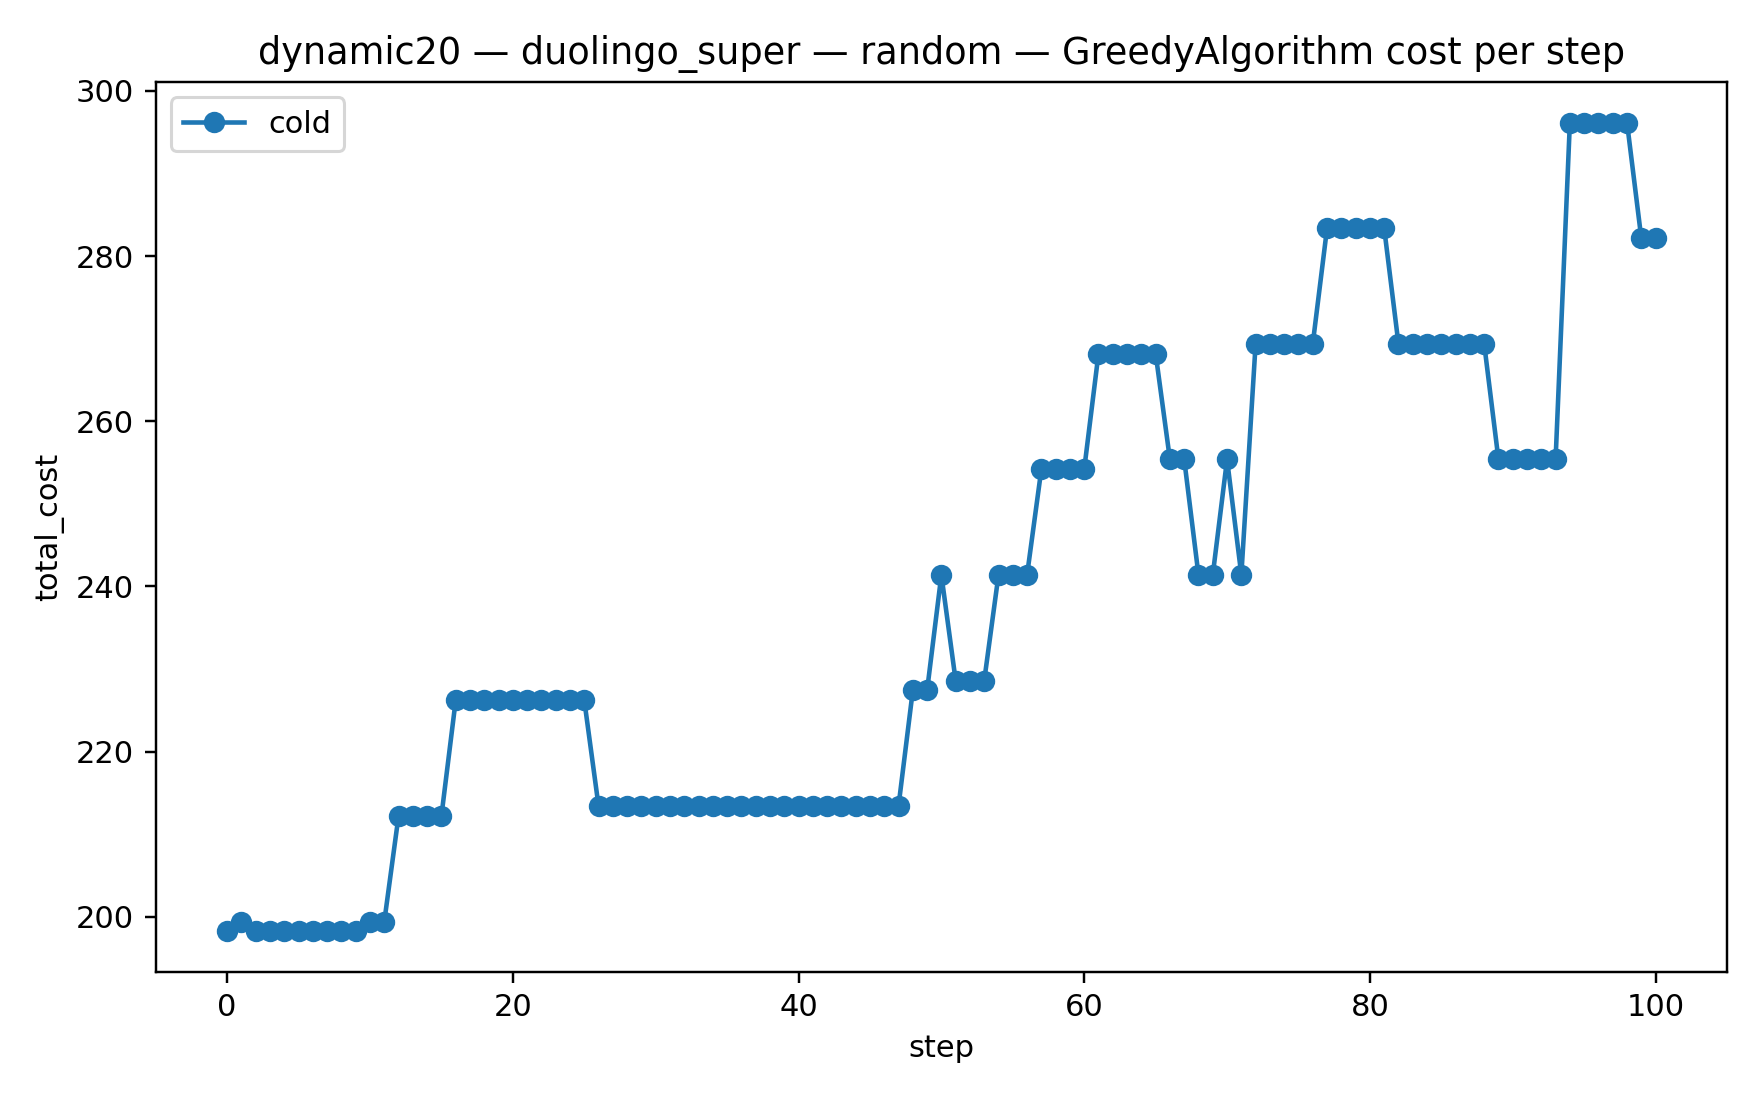
\includegraphics[width=0.48\linewidth]{assets/figures/dynamic/dynamic20/duolingo_super/random/GreedyAlgorithm_cost_per_step.png}
  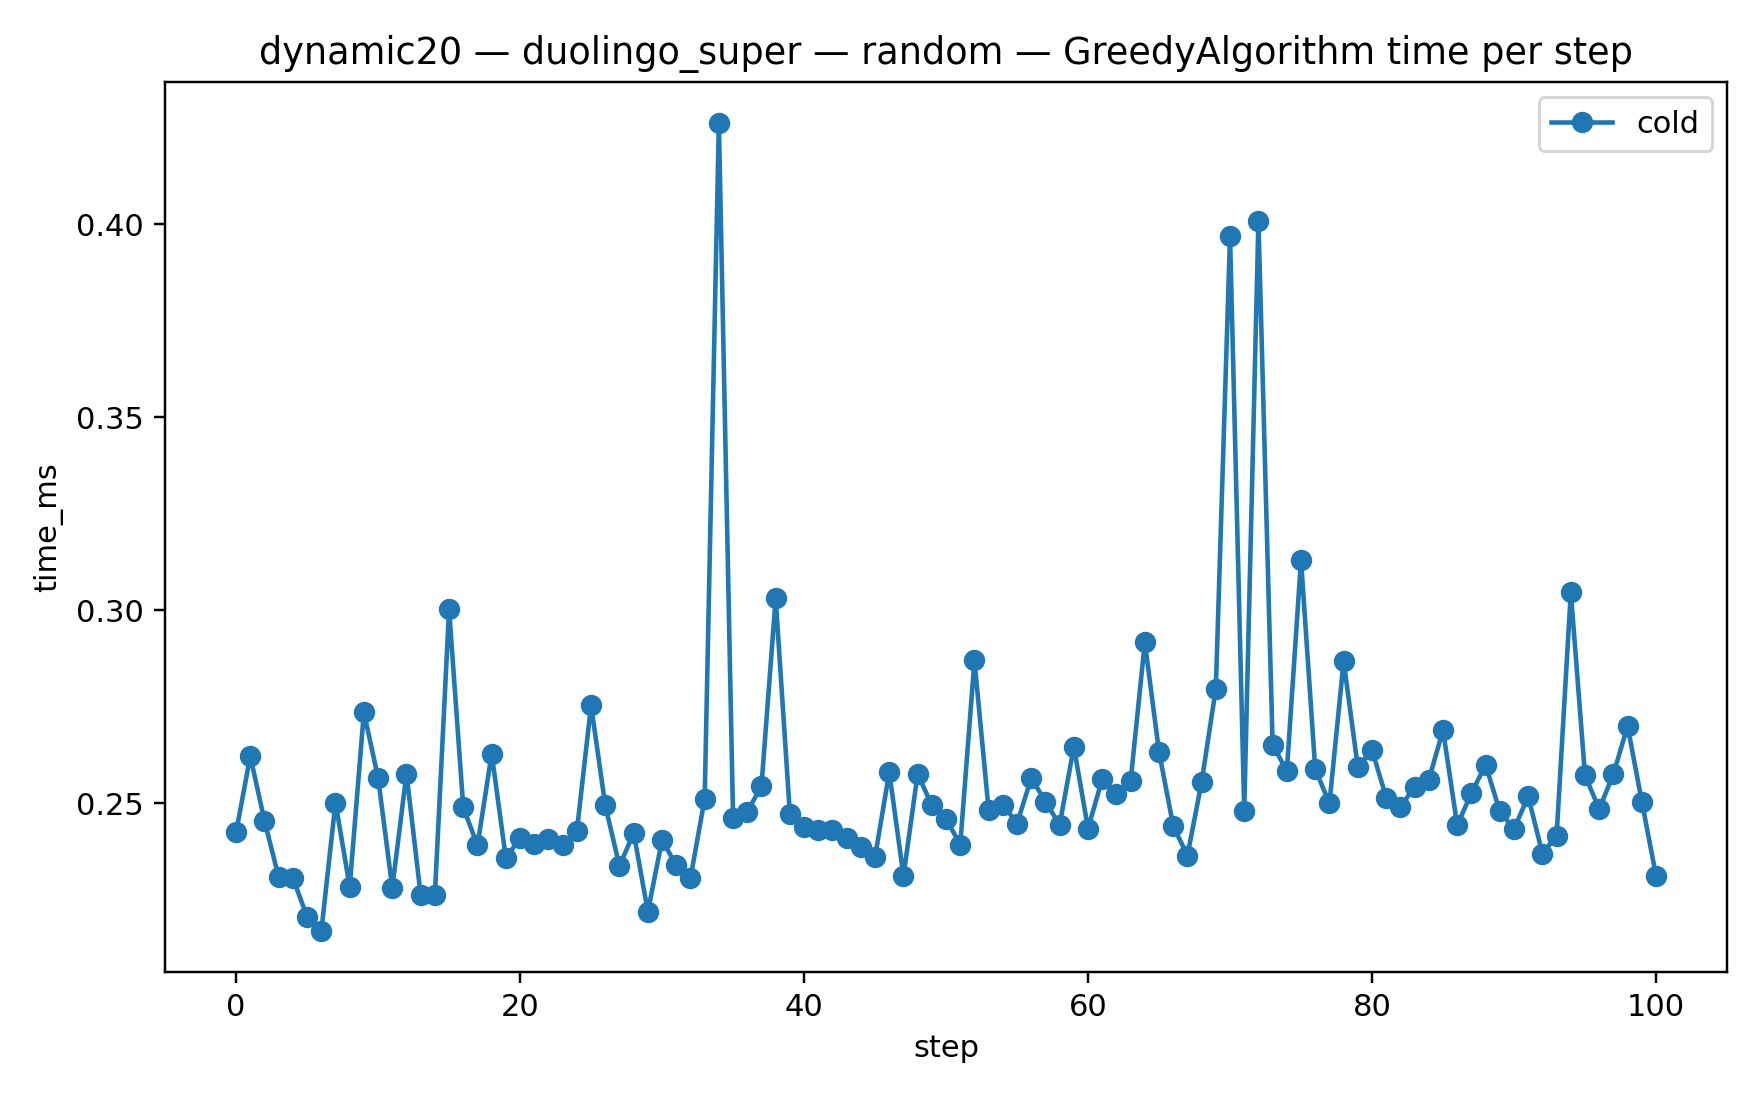
\includegraphics[width=0.48\linewidth]{assets/figures/dynamic/dynamic20/duolingo_super/random/GreedyAlgorithm_time_per_step.png}
\caption{Algorytm zachłanny (cold): koszt i czas vs krok.}
  \label{fig:dyn20_duo_greedy}
\end{figure}

W serii \texttt{dynamic\_20} zaobserwowano, że koszt na wierzchołek algorytmu zachłannego lekko rośnie w czasie (typowo $\approx$~$+0.9$ pkt między krokiem 0 a 100 dla grafu \texttt{random}), co odzwierciedla narastanie trudności po kolejnych mutacjach. Dla metaheurystyk z warm start (np. algorytm genetyczny) trend jest łagodniejszy, a nawet malejący w medianie, co wskazuje na skuteczniejsze wykorzystanie informacji z poprzedniego kroku.

\subsection{\texttt{full}: \texttt{duolingo\_super}, graf \texttt{small\_world}}

\begin{figure}[H]
  \centering
  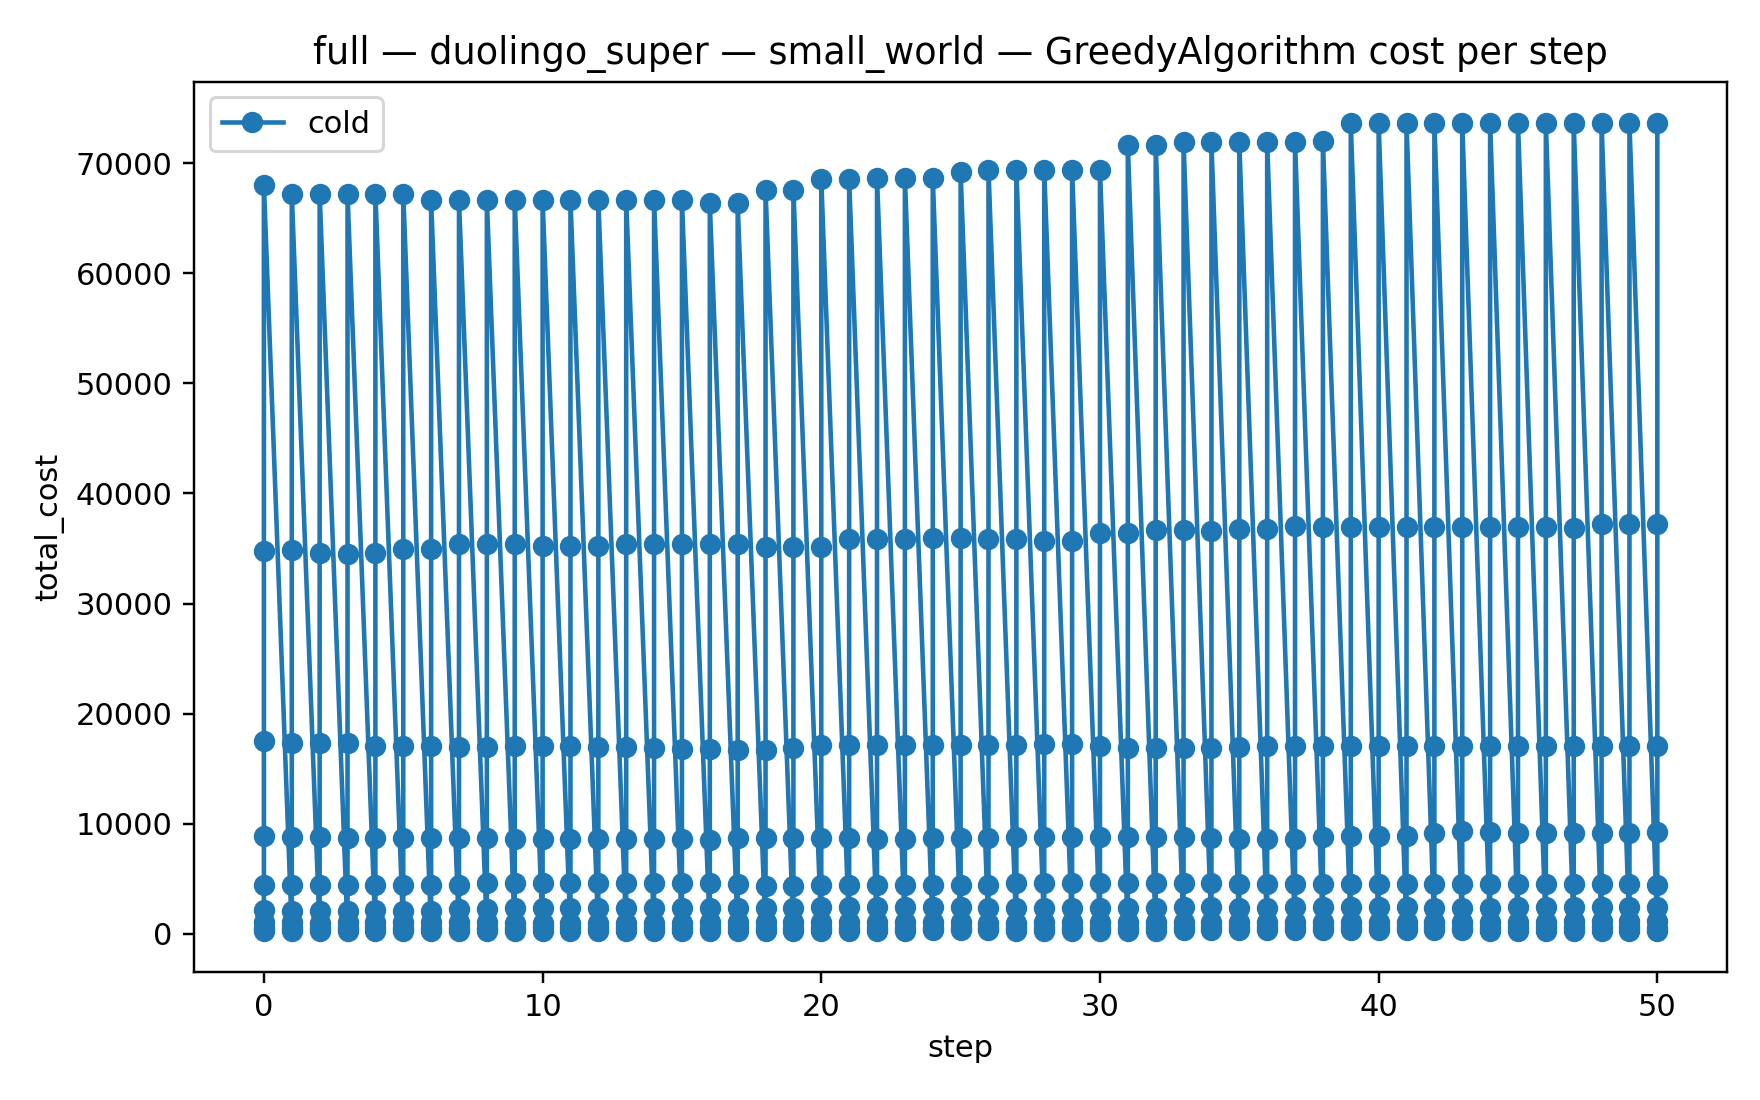
\includegraphics[width=0.48\linewidth]{assets/figures/dynamic/full/duolingo_super/small_world/GreedyAlgorithm_cost_per_step.png}
  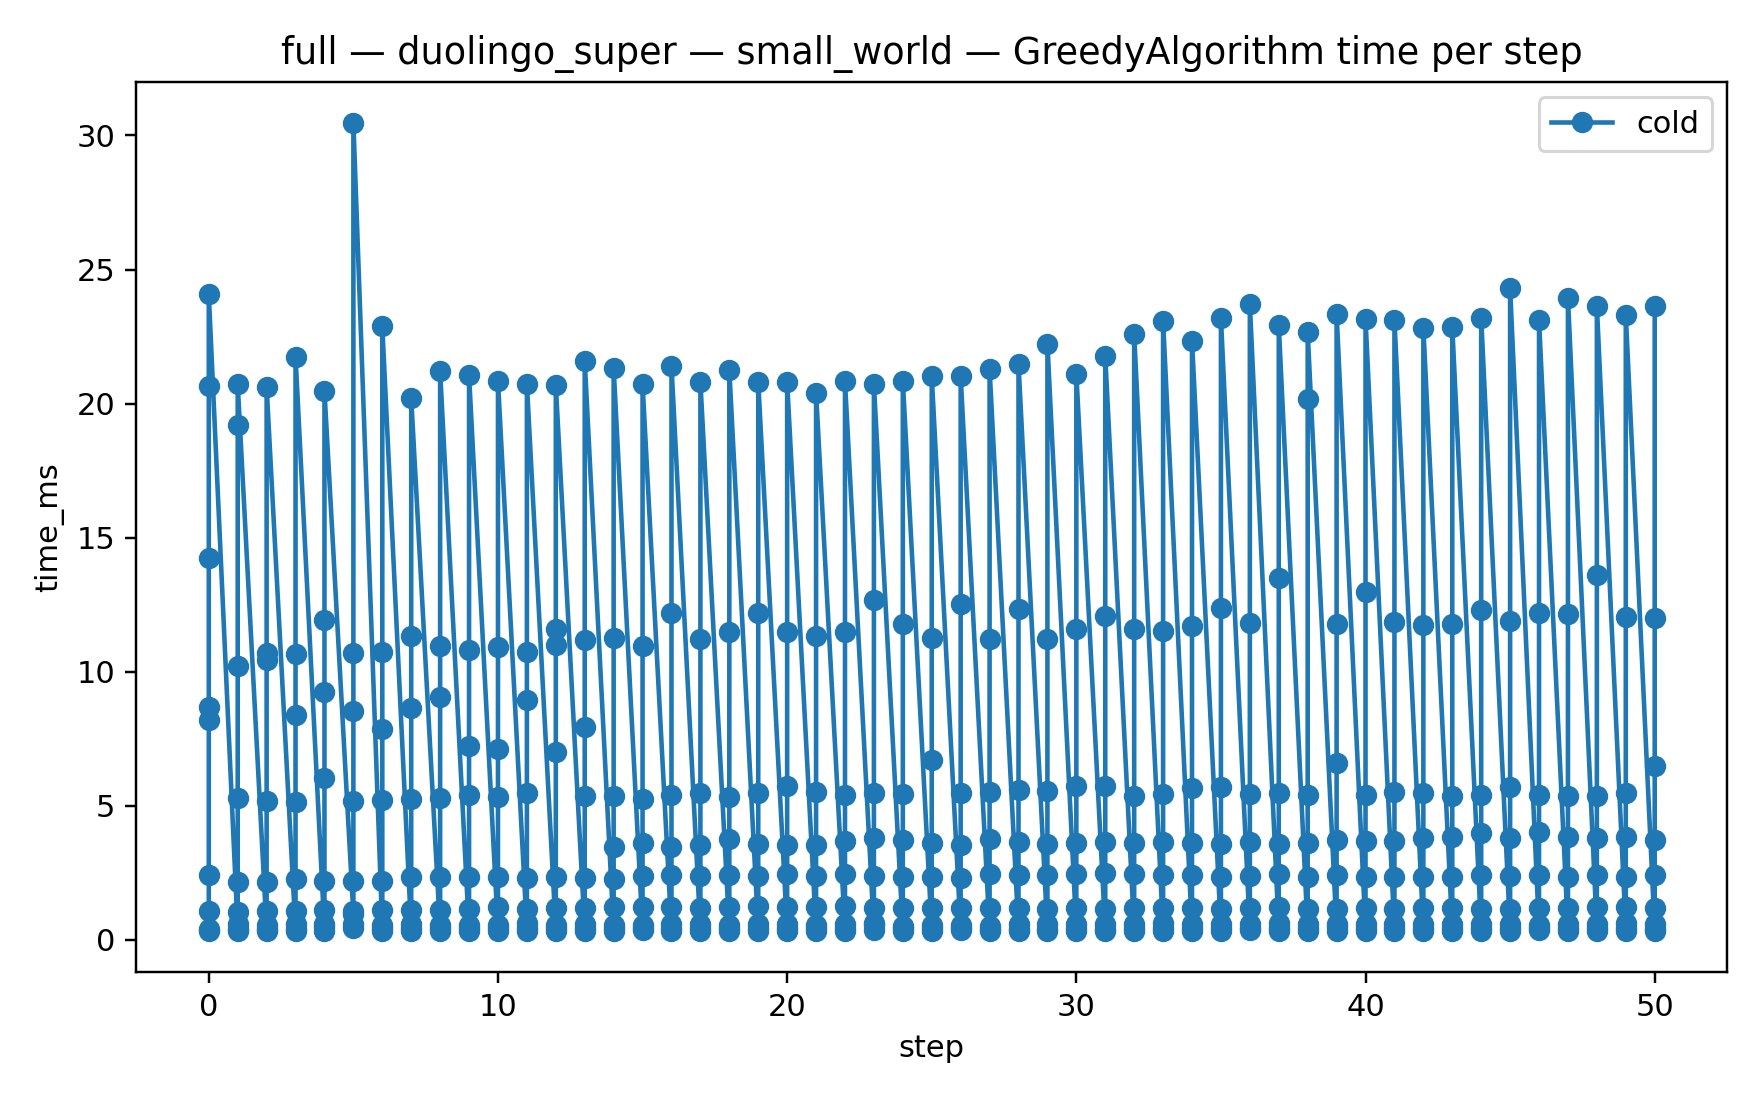
\includegraphics[width=0.48\linewidth]{assets/figures/dynamic/full/duolingo_super/small_world/GreedyAlgorithm_time_per_step.png}
  \caption{Alg. zachłanny (cold): koszt i czas vs krok dla większych $n$.}
  \label{fig:full_duo_greedy}
\end{figure}

Dla większych rozmiarów grafu (seria \texttt{full}) zmiany kosztu na wierzchołek są umiarkowane (mediana rośnie nieznacznie). Czas wykonania pozostaje stabilny w obrębie kroków dla danego rozmiaru, a skokowo rośnie wraz z $n$.

\section{Warianty licencji \texttt{roman\_p\_x} (tylko $n\approx20$)}

W serii \texttt{dynamic\_20} przetestowano czułość na parametr cenowy w konfiguracji \texttt{roman\_domination}. Mediana kosztu na wierzchołek dla algorytmu zachłannego rośnie monotonicznie wraz z parametrem $p$ (przykładowo: \texttt{roman\_p\_1\_5} $\to$ $0.396$, \texttt{roman\_p\_2\_0} $\to$ $0.458$, \texttt{roman\_p\_2\_5} $\to$ $0.522$, \texttt{roman\_p\_3\_0} $\to$ $0.565$ w przekroju wszystkich kroków), co jest zgodne z intuicją — wyższe ceny skutkują wyższymi kosztami końcowymi.

\section{Uwagi metodyczne}

\paragraph{Warm vs cold} W obecnych zestawach dla metaheurystyk zapisywano przebiegi z warm start, natomiast dla algorytmów bez wsparcia warm — przebiegi cold. Wobec braku par ``warm/cold'' w tych samych ustawieniach nie raportowano bezpośredniej różnicy warm–cold na poziomie kroku; zamiast tego pokazano trajektorie czasowo–kosztowe dla każdego algorytmu osobno.

\paragraph{Agregacja kroków} Wykresy kosztu/czasu przedstawiają mediany wartości w danym kroku (jeśli było więcej niż jedno uruchomienie dla kroku), co ogranicza wpływ wartości odstających. Intensywność mutacji liczona jest jako średnia liczba zmian (dodane/uszunięte wierzchołki i krawędzie) przypadająca na wiersz danych w danym kroku.

\paragraph{Ograniczenia obliczeniowe} Dla bardzo dużych $n$ ograniczono zestawy licencji do \texttt{duolingo\_super} i \texttt{roman\_domination}. W tym rozdziale pominięto konfigurację \texttt{spotify} (zostanie omówiona jako rozszerzenie w kolejnym rozdziale).

\section{Wnioski}

\begin{itemize}
  \item Mutacje grafu o umiarkowanej intensywności prowadzą do stopniowego wzrostu trudności; proste heurystyki (np. zachłanna) wykazują lekki wzrost kosztu w czasie.
  \item Metaheurystyki z warm start stabilniej utrzymują koszt (w części przypadków obniżają medianę kosztu na wierzchołek w dłuższym horyzoncie), co potwierdza użyteczność reużycia poprzedniego rozwiązania.
  \item Różnice między rodzinami grafów pozostają zgodne z obserwacjami ze scenariusza statycznego: grafy bezskalowe ułatwiają tworzenie większych grup (niższy koszt na wierzchołek), podczas gdy małoświatowe i losowe są bardziej wymagające.
  \item Zmiany parametrów cenowych w konfiguracji \texttt{roman\_domination} (seria \texttt{roman\_p\_x}) przekładają się wprost na poziom kosztów — wzrost $p$ zwiększa koszt na wierzchołek w całym przebiegu.
\end{itemize}

Podsumowując, symulacja dynamiczna odzwierciedla realistyczny scenariusz zmian w sieci użytkowników i potwierdza, że warto stosować metaheurystyki z inicjalizacją warm, które lepiej wykorzystują ciągłość w czasie, utrzymując niższy koszt przy stabilnym czasie wykonania.
